\subsection{Modelos de regresión}
        
    Un modelo de regresión involucra los siguientes componentes:
    \begin{itemize}
        \item Variable dependiente: Se observan en los datos y se denotan como $Y_i$.
        \item Variables independientes: Se observan en los datos y están definidos en forma de vector $X_i$.
        \item Parámetros desconocidos: Denotados como el vector $\beta$. 
        \item Error cometido: Denotado como el escalar $e_i$.
    \end{itemize}
    
    Se define generalmente entonces, el siguiente modelo, donde $Y_i$ se define a través del vector muestra $X_i$ y el vector $\beta$, mas el error cometido por la predicción de $f$:
    
    \[ Y_i = f(X_i,\beta) + e_i \]
    
    El objetivo al definir este modelo es el de encontrar la mejor función $f$, junto con el parámetro $\beta$, que mejor se ajusten a los datos, en este caso los $Y_i$. Para esto, primero se debe definir la función f, por ejemplo, observando el tipo de relación que tienen los $X_i$ con $Y_i$.
    
    Para la elección de esta función, decidimos descomponerla en una suma de funciones, como primer opción para determinar una función que refleje bien la relación entre las variables. Luego, pensamos en la descomposición de la siguiente manera, partiendo de la expresión inicial dicha anteriormente:
    
    \[ Y_i = f(X_i,\beta) + e_i = f_1(X_{i1},\beta_1) +\ldots + f_n(X_{in},\beta_n) + e_i = \sum_{j=1}^{n} f_j(X_{ij},\beta_j) + e_i\]
    
    Donde cada $X_{ij}$ es una variable independiente dentro del vector, y entonces cada $f_j$ termina siendo la que representa lo mejor posible la relación entre la variable $X_{ij}$ e $Y_{i}$. El problema se convierte ahora en proponer las mejores funciones tal que cada una modele esa relación entre par de variables, y luego de definirlas, ajustar el vector $\beta$.
    
    Para todo el análisis que sigue utilizamos,  regresores por proyección, regresores lineales y polinomiales.. También aplicamos sobre cada uno de los anterior el concepto de regresor segmentado.
      
    \subsubsection{Regresión por proyección}
        
        Definimos primero un modelo simple para trabajar, el cual se basa en la función identidad. Este toma cada variable, y la \textit{proyecta} en la función $f$, es decir:
        
        \[f_j(X_{ij}) = X_{ij}\]
         
        Y luego, utilizando esta definición, se tiene como resultado una función $f$ de la forma:
        
         \[ 
        Y_i 
        = f(X_i,\beta) + e_i 
        = \sum_{j=1}^{n} (\beta_{j} {X_{ij}})  + e_i\]
        
        Como se observa, esta es la idea mas simple para diseñar un modelo, sumando todos los predictores para generar el modelo final. Esta simpleza permite un análisis sencillo, sin tener funciones complicadas involucradas, para entender mejor como se relacionan linealmente los predictores con la variable a explicar.
    \subsubsection{Regresión lineal}
        
        Introdujimos un cambio a las funciones $f_j$ del regresor anterior, para llevarlas a funciones lineales. De esta manera, quedan definidas las funciones como:
        
        \[f_j(X_{ij}) = \beta_{j2} {X_{ij}} + \beta_{j1}\]
        
        La idea atrás de esta forma de la $f$ es la de ver como resulta un modelo simple como el anterior, extendiéndolo a una función lineal para permitir un poco mas de libertad. Este cambio permite moverse de a poco a sofisticaciones del modelo. Luego, la $f$ resultante de esto es:
        
         \[ 
        Y_i 
        = f(X_i,\beta) + e_i 
        = \sum_{j=1}^{n} (\beta_{j2} {X_{ij}} + \beta_{j1})  + e_i\]
        
    \subsubsection{Regresión polinomial}
        
        La regresión lineal es una forma básica y efectiva para definir un modelo inicial, pero tiene sus limitaciones, mas cuando los datos presentan una relación cuadrática quizás, la cual la lineal no llega a capturar. Para la construcción del modelo entonces, introdujimos una mejora con respecto a la anterior, permitiendo que las $f_j$ no sean únicamente lineal, sino un polinomio de grado a definir. De manera análoga al caso anterior, podemos ver esto como:
        
        \[f_j(X_{ij}) = \beta_{jn} {X_{ij}^n} + \beta_{jn-1} {X_{ij}^{n-1}} + \ldots + \beta_{j2} {X_{ij}^2} + \beta_{j1} X_{ij}\]
        
        Notar que esta nueva definición no involucra solo a un $\beta_j$, a diferencia de la definición del principio, donde cada función se encontraba multiplicada por un coeficiente del vector $\beta$. La razón de esta nueva forma de definir la formula general es la de permitir mas libertad para ajustar los parámetros. Con esto, permitimos mas grados de libertad para que cada $X_{ij}$ describa lo mejor posible al $Y_{i}$, y a su vez un ajuste granular sobre cada termino del polinomio. Si no se hiciera esto, tendríamos un solo coeficiente para ajustar a todo el polinomio. Si bien eso puede resultar efectivo, seria equivalente a tener uno por termino, donde todos valen lo mismo, pero con este cambio se permitiría llegar a un ajuste mas fino y probablemente mejor.
        Entonces, con este pequeño cambio sobre la construcción de la función $f$, tenemos:
        
        \[ 
        Y_i 
        = f(X_i,\beta) + e_i 
        = \sum_{j=1}^{n} f_j(X_{ij},\beta_j) + e_i 
        = \sum_{j=1}^{n} (\beta_{jn} {X_{ij}^n} + \ldots + \beta_{j1} X_{ij}) + e_i 
        = \sum_{j=1}^{n} (\sum_{k=1}^{g}\beta_{jk} {X_{ij}^k})  + e_i\]
        
        Siendo $g$ el grado del polinomio a definir.

    \subsubsection{Regresión segmentada}
        
        Generalmente, intentar de explicar la relación entre distintas variables resulta demasiado complejo para un único modelo. Entonces, si se eligen subconjuntos adecuadamente, modelos que solo tengan en consideración esta partición, puede terminar siendo más preciso. Esto se debe a que, en conjuntos de datos reducidos, las relaciones existentes, pueden hacerse más evidentes, si estos datos están relacionados entre si.
        
        Ejemplos de estos segmentos incluyen a las variables categóricas, que son aquellas cuyos valores no están relacionados de una manera que se pueda cuantificar; a las variables numéricas cuantizadas, que consiste en \emph{bucketizar} las mismas, según una división adecuada; y por último a la variable que se intenta predecir.
        
        Una demostración del uso de segmentos puede verse a continuación en la figura (\ref{segs}). En este caso, se intenta estimar los valores de una muestra que se comporta como una función cuadrática. Se puede ver que, al tener en cuenta un único modelo, la mejor resulta una función constante. En cambio, si el conjunto de datos se segmenta según el valor de la característica $x$ (si es mayor o menor a 0), como resultado obtenemos dos modelos. A la hora de predecir, se elige un modelo según el segmento al que pertenezca la muestra a predecir.
        
        
    \begin{figure}[H]
    \centering
        \begin{subfigure}{.3\textwidth}
            \centering
            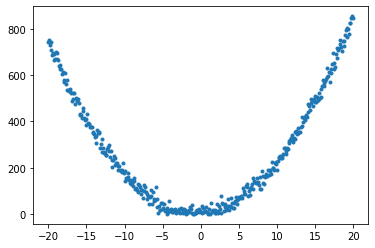
\includegraphics[scale=.35]{img/explicaciones/1_seg.png}
            \caption{Gráfico del conjunto de datos}
        \end{subfigure}
        \begin{subfigure}{.3\textwidth}
            \centering
            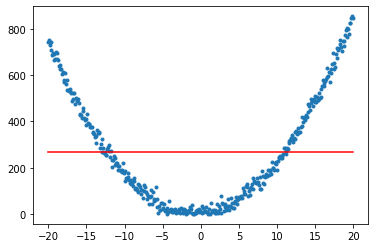
\includegraphics[scale=.35]{img/explicaciones/2_seg.png}
            \caption{Regresor, sin segmentar}
        \end{subfigure}
        \begin{subfigure}{.3\textwidth}
            \centering
            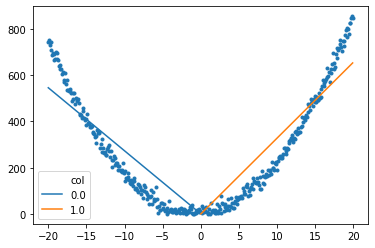
\includegraphics[scale=.35]{img/explicaciones/3_seg.png}
            \caption{Regresor, segmentando}
        \end{subfigure}
        \caption{Ejemplos de modelos con y sin segmentación}
        \label{segs}
    \end{figure}
        
        %Cuando se desea hacer una regresión, se tiene un conjunto de datos, llamadas muestras, los cuales tienen variables independientes involucradas.
        
        %Estas variables, para el caso particular que tratamos, son los \textit{metros cubiertos}, \textit{la cantidad de baños}, etc. Estas variables son numéricas, y reflejan una cantidad de algo.
        
        %Pero por el otro lado, también se tienen la \textit{ciudad}, la \textit{provincia}, etc. A diferencia de las anteriores, estas son variables \textit{categóricas}, y 2 valores distintos de alguna de ellas no tiene ninguna relación.
        
        %Si bien solo se pueden utilizar variables numéricas de manera directa para los regresores explicados hasta ahora, hay una forma distinta de construir un regresor, utilizando la técnica de segmentación.
        
        %La segmentación busca separar las muestras en base a los valores de una variable independiente, ya sea numérica o categórica. Luego, al tener las muestras divididas en grupos, se aplica el \textit{fitting} a cada grupo, obteniendo así un regresor por cada valor de la variable independiente utilizada para segmentar. Aplicando esta técnica a un regresor lineal por ejemplo, se obtiene lo que se llama un regresor lineal segmentado, el cual se muestra a continuación:
    
        Esta técnica tiene como objetivo poder establecer una mejor relación entre la variable a describir y las utilizadas para describirla. En este caso, se puede observar que, segmentar según el signo de la variable $x$, resulta ser beneficioso. Una aclaración que vale la pena mencionar, es que, aunque nos estemos refiriendo a la misma variable $x$, podría pensarse como que la misma se dividió en dos, la variable $x_{<0}$, que se tiene en consideración para un modelo, y la variable $x_{>0}$, que se tiene en consideración en el otro.

        Es importante notar que, no siempre será beneficioso aplicar segmentación sobre los datos. Por ejemplo, si las muestras resultantes luego de segmentar no poseen una cantidad de datos significativa, esto puede causar un \emph{overfitting}. Esto se debe a que, cuando las relaciones subyacentes no están bien definidas, segmentar no aporta un beneficio, y la conclusión es que estamos entrenando nuestros modelos con menos datos.